\chapter{Marco teórico}

% \customEpigraph{Begin at the beginning, the King said gravely, <<and go on till you come to the end: then stop.>>}{Fulano de Tal, \textit{Título del libro}}



\section{Inteligencia artificial, aprendizaje automático y aprendizaje profundo}
\todo{Reformar esta sección para incluir la IA generativa y establecer las relaciones con el resto de conceptos}

Comencemos por definir las diferentes disciplinas que intervienen en el estudio y desarrollo de sistemas de inteligencia artificial. A menudo se encuentran términos como \gls{ia}, \gls{ml} o \gls{dl} usados de forma intercambiable. Sin embargo, cada uno tiene un significado específico, y es crucial diferenciarlos para comprender el estado actual de la investigación en el área. Estos conceptos se organizan jerárquicamente \citep{torresivinalsPythonDeepLearning2020}, donde la  \gls{ia} es el término más general, que abarca el \gls{ml}, y este último incluye al \gls{dl} (ver Figura \ref{fig:ai_ml_dl}).

\begin{figure}[H]
    \caption[Relación entre IA, ML y DL]{Relación entre IA, ML y DL}
    \centering
    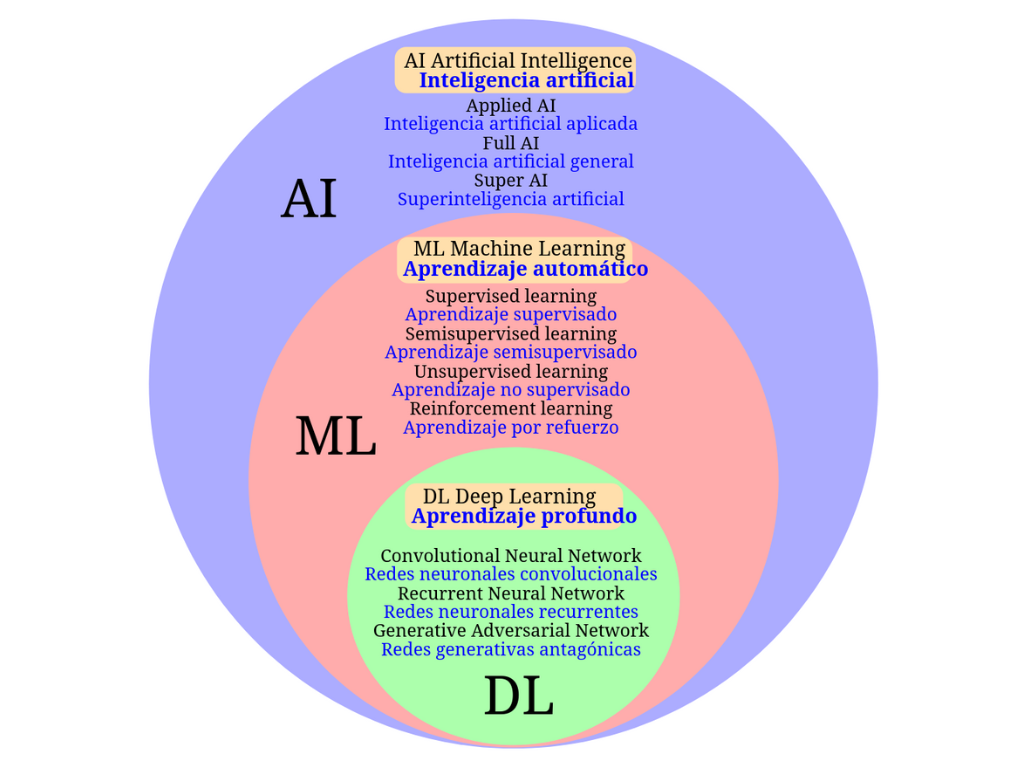
\includegraphics[width=0.8\textwidth]{./figuras/AI_ML_DL.png}
    \source{Jzh2074 \protect\citeyear{jzh2074}, Wikimedia Commons; Wang et al. \protect\citeyear{wang2021promising}.}
    \label{fig:ai_ml_dl}
\end{figure}

% He añadido una imagen de relación AI, ML, DL y AI generativa. Sería interesante modificar lo anterior para hablar también de la IA generativa, que al fin y al cabo es la que nos interesa. La imagen la he sacado de aquí: https://medium.com/@kitkat73275/introduction-to-generative-ai-833c9c467dfa (añadirla a bibliografía y citarla)


La \gls{ia} es el campo de estudio más antiguo entre los tres, y no se limita únicamente al ámbito computacional. En su sentido más amplio, la \gls{ia} ha sido abordada por la filosofía. Los racionalismos y estructuralismos, fundamentales en los sistemas de pensamiento occidentales, forman la base conceptual de la inteligencia artificial. Sin embargo, no es hasta el siglo XX cuando se empieza a considerar la posibilidad matemática de un sistema que genere inteligencia. En 1950, Alan Turing publicó su artículo \textit{Computing Machinery and Intelligence} \citep{alan1950a}, en el que propuso un test para determinar si una máquina puede pensar. Este test, conocido como <<Test de Turing>>, consiste en la interacción de un humano con una entidad artificial usando solo un terminal de texto como interfaz. La máquina aprueba el test si el humano no puede discernir si está interactuando con una entidad artificial o humana. A pesar de sus limitaciones y su enfoque antropocéntrico sobre la inteligencia, este test sigue siendo una referencia común para evaluar sistemas modernos de \gls{ia}.

No obstante, el concepto de \gls{ia} trasciende la mera imitación humana, aunque no lo descarta. Si consideramos la <<racionalidad>> como un conjunto de estructuras lógicas que incluyen el pensamiento y el razocinio humanos, la \gls{ia} no necesita limitar su objetivo a superar el test de Turing. Las definiciones de \gls{ia} a lo largo del tiempo han variado dependiendo de si se enfocan en imitar el pensamiento o acción <<humanos>> o el pensamiento y acción <<racional>> \citep{RussellStuartJ2021AI:A}.

Además de a Alan Turing, debemos a Curt Gödel los fundamentos matemáticos de los procesos de pensamiento, considerados sistemas computacionales capaces de generar \textit{outputs} racionales a partir de \textit{inputs} arbitrarios. La idea de que el cerebro humano es una de las posibles <<máquinas de Turing>> \citep{penroseNuevaMenteEmperador2015} ha sido un estímulo para la investigación en \gls{ia} computacional. Además, investigaciones en <<procesamiento del lenguaje natural>>, en las que destaca el concepto de <<entropía>> de Shannon \citep{shannon1951prediction} y que han acompañado el desarrollo de lenguajes de programación, son fundamentales para los sistemas actuales de \gls{ia}.


\section{\textit{Machine Learning}}

El \gls{ml}, o \textit{aprendizaje automático}, es una subdisciplina de la \gls{ia} que investiga algoritmos y modelos matemáticos que habilitan a un sistema computacional a aprender a partir de datos sin ser explícitamente programado. Estos sistemas identifican patrones y toman decisiones con poca o sin intervención humana. En el \gls{ml}, el modelo se autoconfigura basándose en los datos con los que se entrena. Las únicas intervenciones humanas son el diseño de la arquitectura y la provisión de los datos de entrenamiento, aunque incluso estas tareas podrían delegarse a otro sistema de \gls{ml} en determinadas circunstancias.

Aunque el \gls{ml} ha sido una área de interés desde los inicios de la computación, es esencial reconocer que es solo una faceta de la \gls{ia}. No todos los sistemas inteligentes son sistemas de \gls{ml}. Por ejemplo, el software de ajedrez \textit{Deep Blue} de IBM, que venció al campeón mundial Garry Kasparov en 1997, no se basaba en \gls{ml} \citep{campbellDeepBlue2002}. En lugar de ello, \textit{Deep Blue} utilizaba una vasta base de datos de jugadas de ajedrez y algoritmos de búsqueda eurísticos para decidir el mejor movimiento en cada situación. Otros sistemas no basados en \gls{ml}, como los <<sistemas expertos>>, utilizan reglas predefinidas para tomar decisiones y se aplican ampliamente en áreas como medicina, ingeniería y gestión empresarial.

En términos generales, el objetivo del \gls{ml} es encontrar una función matemática que describa un conjunto de datos de entrenamiento y que, posteriormente, pueda prever datos desconocidos con precisión. Esta capacidad predictiva se conoce como <<inferencia>>. El proceso busca que la función determinada durante el entrenamiento aproxime la función real que describe los datos, permitiendo al sistema generalizar de forma análoga al cerebro humano.

Se utiliza el término <<modelo>> para referirse al sistema una vez que ha sido entrenado y posee capacidad predictiva. Dependiendo de su aplicación, un modelo puede ser empleado para predecir datos desconocidos o clasificarlos. Si produce un valor numérico, se habla de <<regresión>>; si categoriza datos, de <<clasificación>>. La clasificación puede ser binaria o multiclase, y la regresión unidimensional o multidimensional.

El aprendizaje en \gls{ml} se produce a través de un proceso de entrenamiento. Según la naturaleza de los datos y el método de validación, existen tres tipos principales de aprendizaje automático \citep[p. ~38]{torresivinalsPythonDeepLearning2020}:

\begin{itemize}
    \item \textbf{Aprendizaje supervisado:} Aquí, los datos se etiquetan con la respuesta esperada, como imágenes de animales etiquetadas como <<gato>> o <<perro>>. Tras el entrenamiento, se espera que el sistema identifique imágenes no etiquetadas correctamente. Este procedimiento de aprendizaje e inferencia queda reflejado en la Figura \ref{fig:labeled_data_training}. Una de las aplicaciones más comunes del aprendizaje supervisado es la clasificación de imágenes. Sin embargo, su debilidad consiste precisamente en la necesidad de etiquetado de los datos de entrenamiento, que puede ser un proceso costoso y laborioso si este solo se puede hacer manualmente.
    
    \item \textbf{Aprendizaje no supervisado:} En este caso, los datos no están etiquetados. El sistema busca patrones y agrupa datos en categorías por sí mismo. Precisamente este es el tipo de aprendizaje utilizado en el entrenamiento de modelos de lenguaje, donde los datos de entrenamiento son textos sin etiquetar.
    
    \item \textbf{Aprendizaje por refuerzo:} El sistema aprende interactuando con un entorno. No recibe etiquetas explícitas, sino recompensas por decisiones correctas y penalizaciones por errores. Este es el modo de aprendizaje más parecido al humano, ya que se basa en la experiencia. Sin embargo, a pesar de ser uno de los métodos más atractivos de aprendizaje automático, es el más complejo de implementar y requiere un entorno de simulación adecuado, que no siempre es posible ni eficiente en términos de computación.
\end{itemize}

\begin{figure}[H]
    \caption[Esquema de aprendizaje supervisado]{Esquema de aprendizaje supervisado, usando datos de entrenamiento etiquetados. En la inferencia se espera que el modelo pueda clasificar datos no etiquetados.}
    \centering
    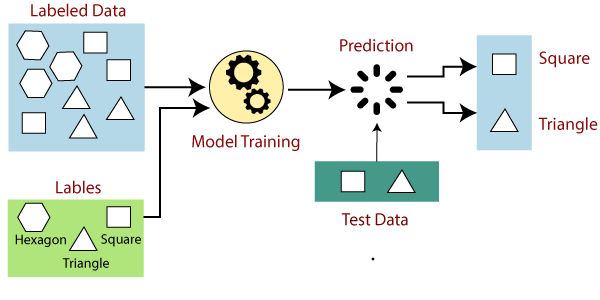
\includegraphics[width=0.4\textwidth]{./figuras/labeled_data_training.png}
    \source{\cite{FindWaysDeal}}
    \label{fig:labeled_data_training}
\end{figure}


\section{Deep Learning}

Esta sección pretende ser una somera introducción a los conceptos de \gls{dl} y \gls{rna}, que constituyen la base de los modelos de lenguaje, objeto de nuestro estudio, con la única finalidad de aportar un aparato teórico mínimo en el que contextualizarlo. En los últimos meses la bibliografía sobre este tema ha crecido exponencialmente. Además de las obras citadas en este trabajo, se puede consultar, a modo de introducción para no especialistas, \cite{BeginnerGuideNeural}. El \gls{dl} es una subdisciplina del \gls{ml} que utiliza redes neuronales artificiales para aprender de forma automática. Las \gls{rna} son modelos matemáticos que imitan el funcionamiento de las neuronas biológicas y hunden sus raíces en la intersección entre biología, matemáticas y ciencias de la computación en la primera mitad del siglo XX....

\subsection{El concepto de neurona artificial}

Para entender el funcionamiento de una \gls{rna} y, por extensión, de un modelo de \gls{dl}, antes es necesario comprender el de la <<neurona artificial>>. Una neurona artificial no es sino un modelo simplificado de una neurona natural que encontramos en el sistema nervioso de los animales. Análogamente a su homóloga biológica, una neurona artificial recibe una serie de entradas, las procesa y devuelve una salida. La entrada de una neurona artificial es la suma ponderada de las salidas de las neuronas de la capa anterior. Esta suma ponderada se pasa a una función de activación, que determina la salida de la neurona. Sin necesidad de entrar en detalles matemáticos, la función de activación más común es la función sigmoide, que devuelve un valor entre 0 y 1 de una forma no lineal. La Figura \ref{fig:neurona_artificial_natural} muestra un esquema de una neurona artificial. 

\begin{figure}[H]
    \caption[Neurona biológica y neurona artificial o <<perceptrón>>]{Neurona biológica y neurona artificial o <<perceptrón>>}
    \centering
    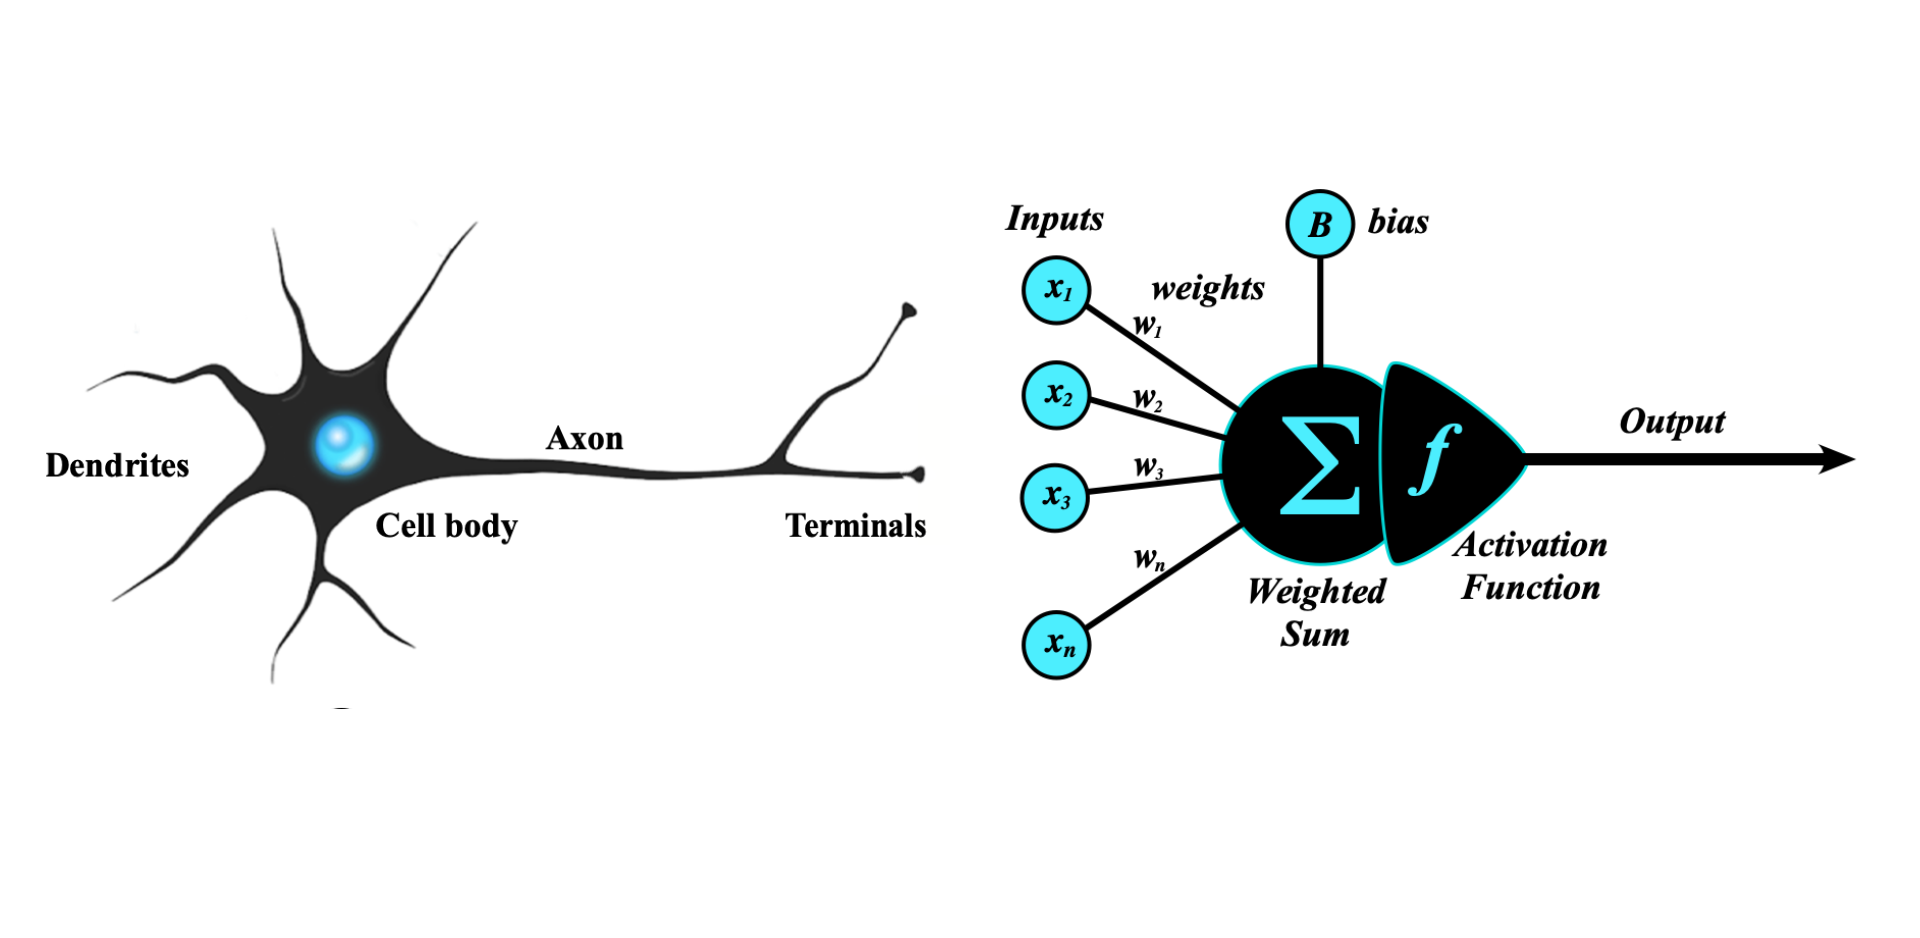
\includegraphics[width=0.4\textwidth]{./figuras/perceptron_with_neuron.png}
    \source{\cite{DeepLearningDL}}
    \label{fig:neurona_artificial_natural}
\end{figure}

Este concepto fue expuesto por primera vez por F. Rosenblatt en 1958 \citep{rothmanTransformersNaturalLanguage2021} bajo el nombre de <<perceptrón>>. El perceptrón no era otra cosa que un modelo de clasificación binaria, es decir, solo puede clasificar datos en dos categorías. Rosenblatt planteo su modelo para ser implementado en hardware, y de hecho se construyó un prototipo en 1959. Sin embargo, el perceptrón tenía limitaciones que no permitían su aplicación a problemas más complejos. Sin embargo, en 1969, Minsky y Papert publicaron un libro \citep{minsky1969perceptrons} en el que demostraban que el perceptrón no podía resolver problemas linealmente no separables. Este hecho supuso un freno en la investigación en \gls{rna}, que no se retomó hasta la década de los 80, cuando se desarrollaron nuevos modelos de redes neuronales artificiales que permitían resolver problemas más complejos. Actualmente sabemos que una red neuronal de varias capas puede aproximar arbitrariamente cualquier función matemática, lo que ha venido a llamarse <<teorema de la aproximación universal>>, propuesto en 1989 por Hornik en su artículo \textit{Multilayer feedforward networks are universal approximators} \citep{hornikMultilayerFeedforwardNetworks1989}. Este teorema tiene grandes implicaciones no solo científicas, sino también filosóficas, en la medida en que podemos considerar que una red neuronal artificial es capaz de imitar el funcionamiento del cerebro humano y su comportamiento, el cual puede reducirse al de una función matemática, por compleja que esta sea. En otras palabras, existe una <<máquina de Turing>> capaz de modelar el cerebro humano. R. Penrose explora las implicaciones de que nuestro cerebro fuera una <<máquina de Turing>> \citep{penroseNuevaMenteEmperador2015}.


\subsection{Redes neuronales artificiales}
Una \gls{rna} es un modelo matemático que se compone de varias capas de neuronas artificiales. La primera capa se denomina <<capa de entrada>> y recibe los datos de entrada. La última capa se denomina <<capa de salida>> y devuelve la predicción del modelo. Las capas intermedias se denominan <<capas ocultas>> y son las que permiten que el modelo pueda aproximar cualquier función matemática. La Figura \ref{fig:deep_neural_network} muestra un esquema de una \gls{rna} con una capa de entrada, dos capas ocultas y una capa de salida.

% La salida de la neurona se pasa a las neuronas de la capa siguiente, y así sucesivamente hasta llegar a la capa de salida. La salida de esta última capa es la predicción del modelo. 

\begin{figure}[H]
    \caption[Estructura de capas de una red neuronal artificial]{Estructura de capas de una red neuronal artificial, con una capa de entrada, dos capas ocultas y una capa de salida.}
    \centering
    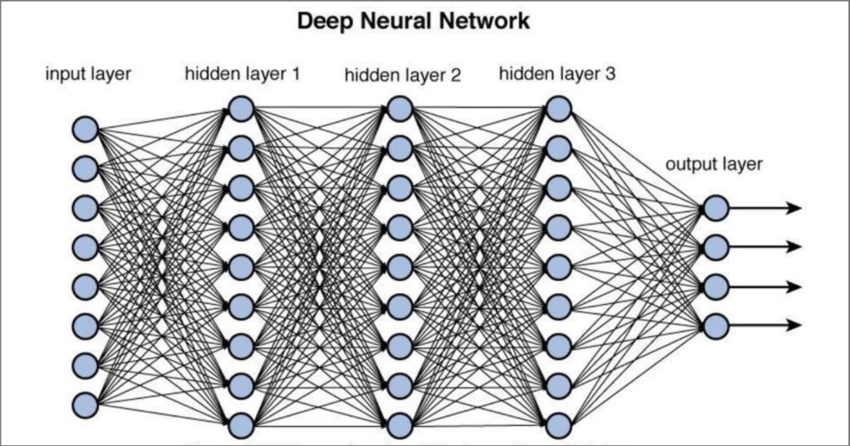
\includegraphics[width=0.4\textwidth]{./figuras/Deep_neural_network.png}
    \source{\cite{zraraPORTFOLIOOPTIMIZATIONUSING2021}}
    \label{fig:deep_neural_network}
\end{figure}

En función de los objetivos de la \gls{rna}, suarquitectura o estructura interna puede variar considerablemente. Una \gls{rna} puede constar de una sola capa, de una capa de entrada y otra de salida y de múltiples capas ocultas. Cada arquitectura busca resolver un tipo de problema concreto. Una arquitectura especialmente compleja, y que ha dado muy buenos resultados en la visión artificial es la \gls{cnn}, inspirada en el funcionamiento de la corteza visual del cerebro humano. Las \gls{cnn} se utilizan para el reconocimiento de imágenes y vídeos, y han sido la base de los avances en el campo de la visión artificial en los últimos años.

Independientemente de su estructura, una \gls{rna} o modelo de \textit{Deep Learning} debe ser entrenado para que pueda aprender a partir de los datos. El proceso de entrenamiento consiste en presentar los datos de entrenamiento a la red neuronal y ajustar los parámetros internos de la red para que la salida se aproxime a la salida esperada. Este proceso se repite iterativamente hasta que la salida de la \gls{rna} se aproxima a la salida esperada con un margen de error aceptable. Una vez entrenada, la \gls{rna} puede predecir la salida de datos desconocidos. Este proceso se ilustra en la Figura \ref{fig:ann_training} Por parámetros internos entendemos los pesos de las conexiones entre neuronas, que son los que en definitiva determinan la salida de la red neuronal. Un modelo antes de ser entrenado da como salida valores aleatorios, y el entreamiento consiste en ajustar estos valores para que la salida se aproxime a lo esperado. Existe una relación, grosso modo, entre la cantidad de parámetros (pesos) de un modelo y su capacidad predictiva, al tiempo que aumenta considerablemente el tiempo de entrenamiento y la capacidad computacional necesaria para entrenarlo. Esta es una de las razones por las que ha habido que esperar a los últimos años para empezar a ver resultados equiparables a los del cerebro humano, especialmente en tareas de generación de imágenes, vídeo, audio o texto.

\begin{figure}[H]
    \caption[Diagrama de entrenamiento de una red neuronal artificial]{Diagrama de entrenamiento de una red neuronal artificial.}
    \centering
    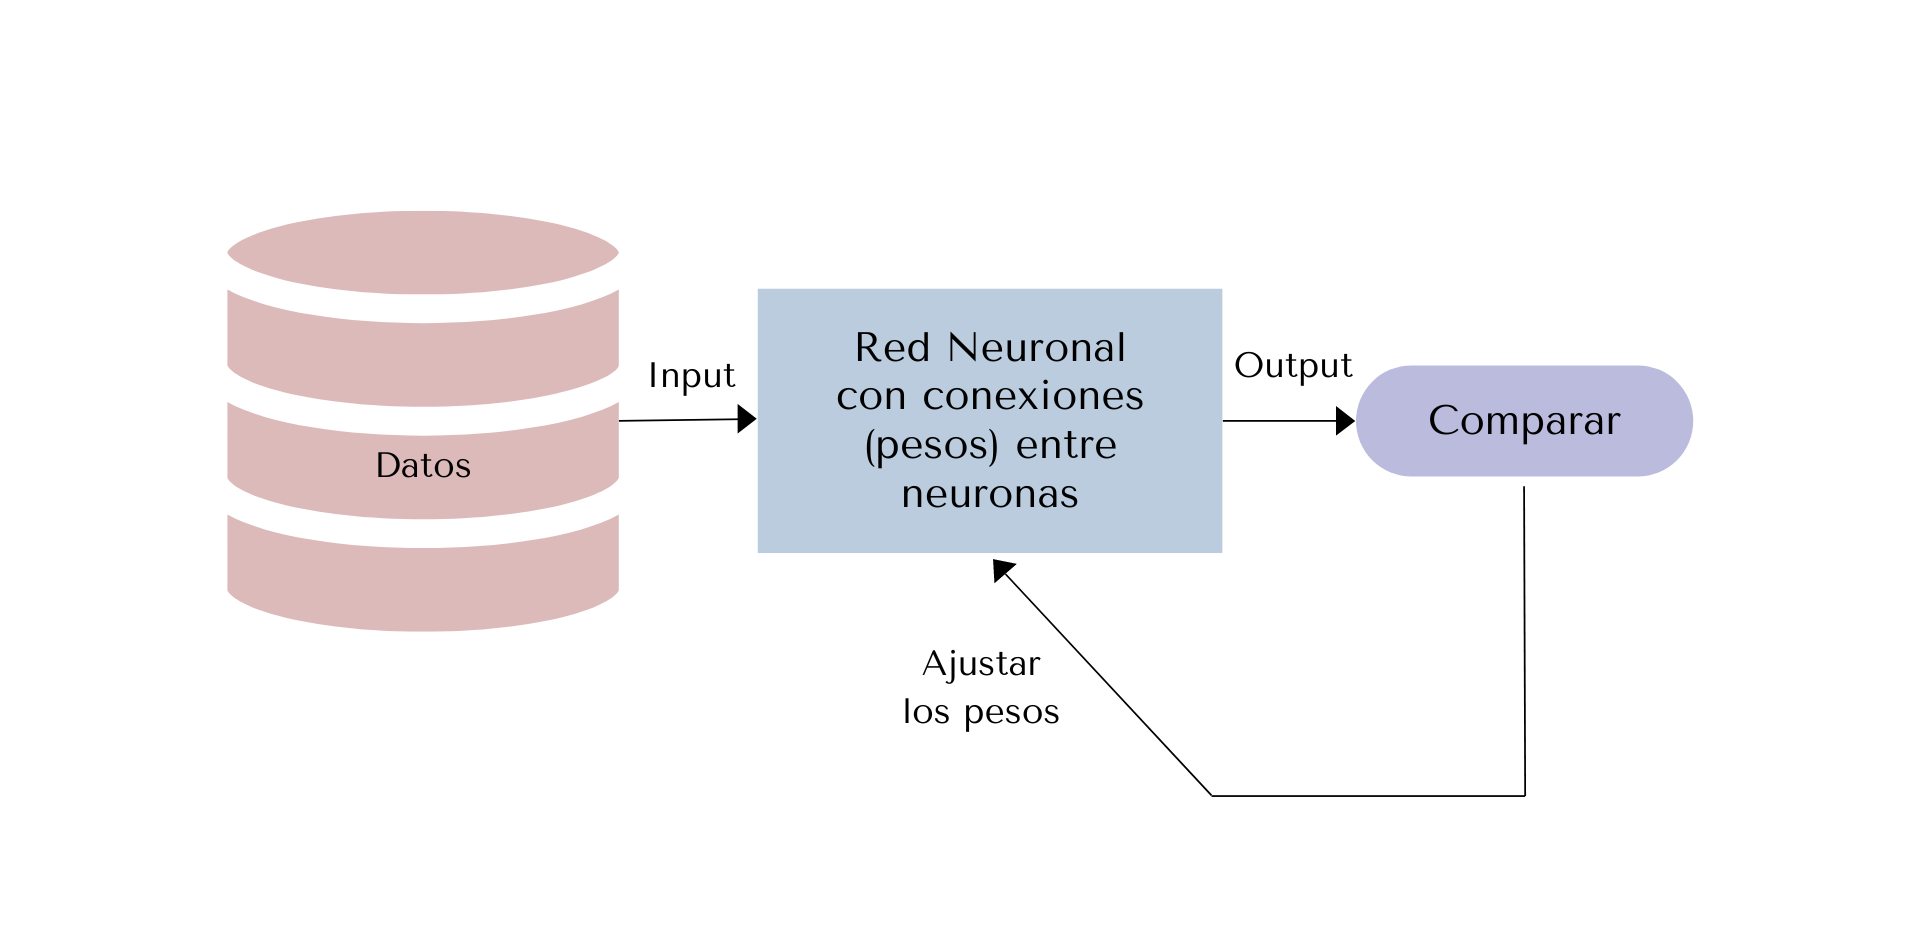
\includegraphics[width=0.9\textwidth]{./figuras/ann_training.png}
    \source{Elaboración propia}
    \label{fig:ann_training}
\end{figure}

\subsection{La arquitectura Transformer}
Hasta 2017, el estado del arte en el ámbito del procesamiento de lenguaje natural por medio de modelos de \textit{Deep Learning} eran las redes neuronales recurrentes (RNN). Estas se basaban en la idea de que la salida de una neurona se podía retroalimentar a la entrada, de forma que la salida de la neurona en el instante $t$ se podía usar como entrada en el instante $t+1$. Esta arquitectura se ilustra en la Figura.... Sin embargo, las RNN presentaban un problema conocido como \textit{vanishing gradient}, que hacía que el modelo no pudiera aprender de secuencias largas. Este problema se solucionó con las redes neuronales de memoria a corto y largo plazo (LSTM), que permitían que la información fluyera a través de la red sin perderse. Sin embargo, las LSTM no podían trabajar con grandes cantidades de tokens de contexto, lo que limitaba su aplicación a tareas de procesamiento de lenguaje natural.

Sin embargo, en 2017, \citeauthor{vaswaniAttentionAllYou2017} publicaron un artículo \citep{vaswaniAttentionAllYou2017} en el que proponían una nueva arquitectura de red neuronal, denominada \textit{Transformer}, que no se basaba en las RNN y que permitía trabajar con grandes cantidades de tokens de contexto. Esta arquitectura se basaba en el concepto de \textit{atención}, que permite que el modelo pueda aprender de secuencias largas. En esta arquitectura, no importa la posición de los tokens de la secuencia de entrada, ya que el modelo aprende a asignar pesos a cada token en función de su relevancia para la predicción del siguiente token. A diferencia de una RNN, un \textit{Transformer} puede procesar todos los tokens de una secuencia de entrada en paralelo, lo que lo hace mucho más eficiente computacionalmente tanto en el entrenamiento como en la inferencia. La Figura \ref{fig:transformer_attention} muestra una matriz de atención de un \textit{Transformer} entrenado con textos en inglés.

En la figura \ref{fig:transformer_architecture} se puede ver un esquema de la arquitectura \textit{Transformer}.

\begin{figure}[H]
    \caption[Aquitectura de Transformer]{Aquitectura de Transformer}
    \centering
    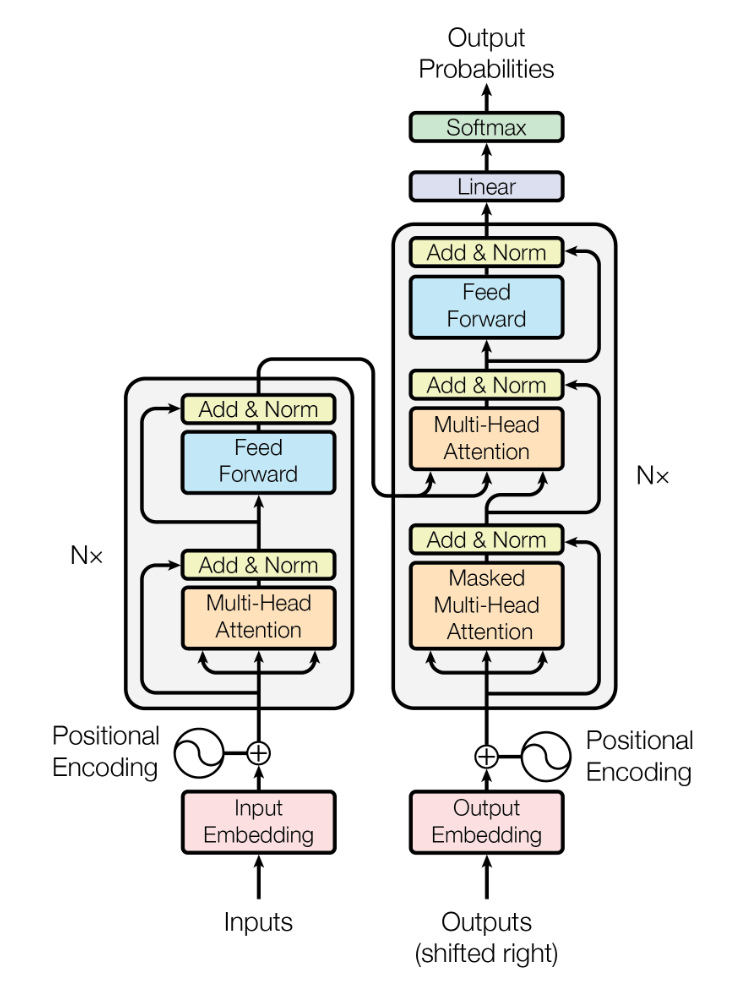
\includegraphics[width=0.4\textwidth]{./figuras/Transformer_architecture.png}
    \source{\cite{vaswaniAttentionAllYou2017}}
    \label{fig:transformer_architecture}
\end{figure}

\begin{figure}[H]
    \caption[Matriz de \textit{atención} de un \textit{Transformer} entrenado con textos en inglés]{Matriz de \textit{atención} de un \textit{Transformer} entrenado con textos en inglés. En ella queda representada la atención de cada token de la secuencia de entrada <<He later went to report Malaysia for one year>> con respecto a los demás.}
    \centering
    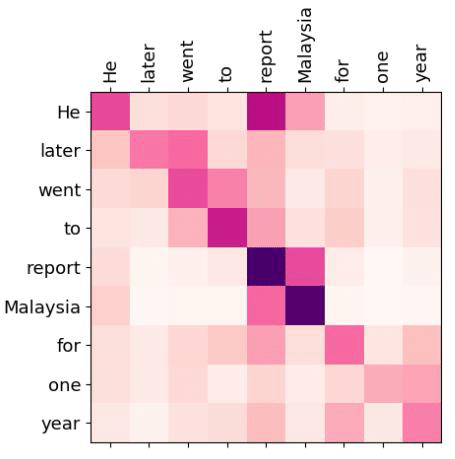
\includegraphics[width=0.4\textwidth]{./figuras/Transformer_attention_matrix.png}
    \source{\cite{duAddressingSyntaxBasedSemantic2022}}
    \label{fig:transformer_attention}
\end{figure}

\section{Modelos de lenguaje}

Un \textit{modelo de lenguaje} es un modelo estadístico que asigna una probabilidad a una secuencia de palabras dada como entrada. Esencialmente, es una función matemática diseñada para simular la forma en que se escribe en lenguaje natural. Una analogía común para entender el funcionamiento de un \textit{modelo de lenguaje} es la función predictiva de un teclado. Mientras escribimos en nuestro dispositivo móvil, el teclado nos sugiere palabras que probablemente seguirán a las ingresadas. Esta capacidad de predicción es el fundamento de los \textit{modelos de lenguaje}, incluyendo chatbots avanzados.

Desde una perspectiva técnica, un \textit{modelo de lenguaje} devuelve como salida la distribución de probabilidad del siguiente \textit{token}, dada una secuencia de \textit{tokens} como entrada \citep{GenerationLLMs}. Un \textit{token} es la unidad mínima de información que el modelo procesa y, generalmente, equivale a una palabra\footnote{Aunque un token suele ser una palabra, también puede ser un signo de puntuación, número o cualquier otra unidad mínima de información.}. La Figura \ref{fig:llm_generation} ilustra un \textit{modelo de lenguaje} que recibe una secuencia de palabras y devuelve la distribución de probabilidad del siguiente \textit{token} después de haber sido entrenado con textos en inglés.

\begin{figure}[H]
    \caption[Inferencia de \textit{token} de un LLM]{Inferencia de \textit{token} de un LLM}
    \centering
    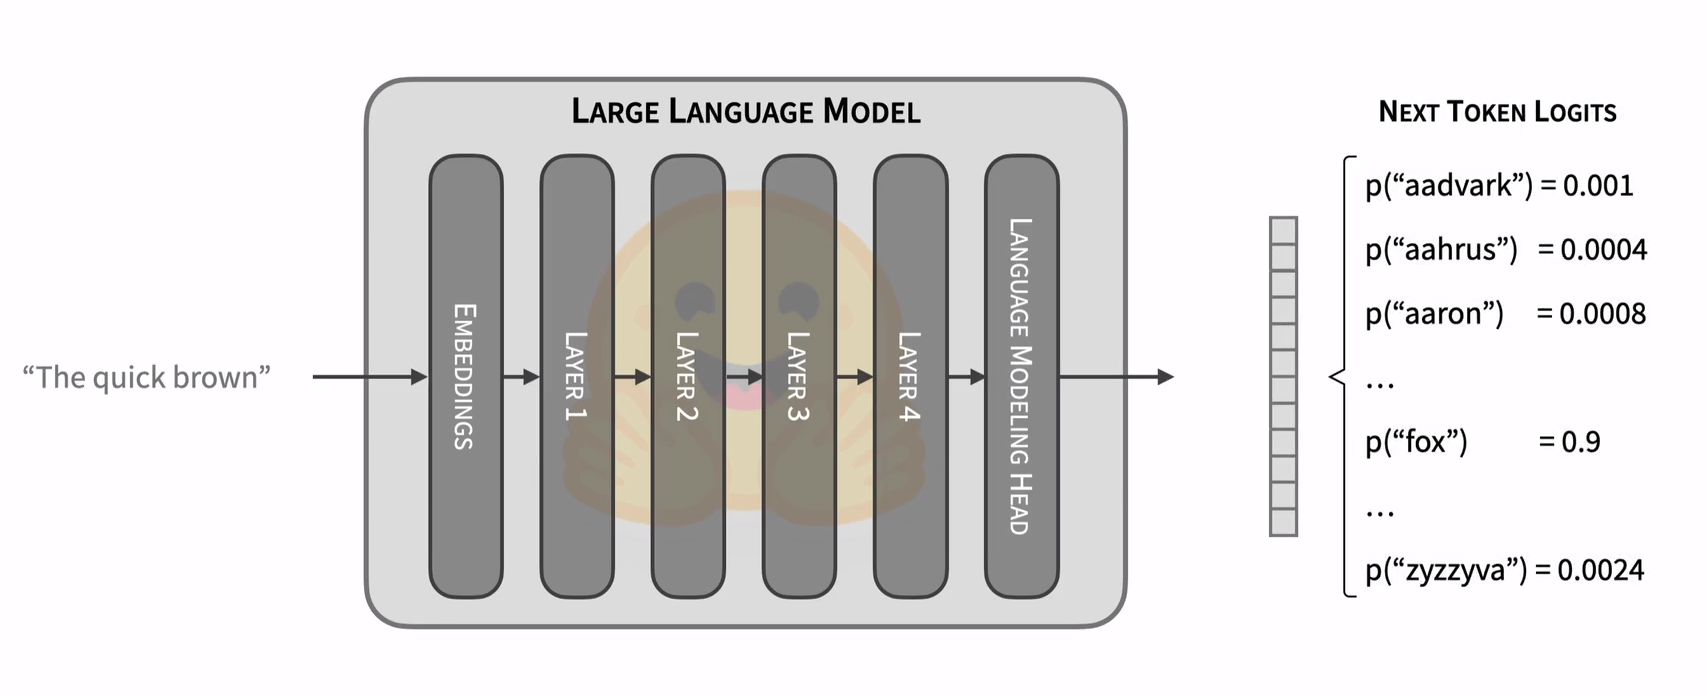
\includegraphics[width=0.9\textwidth]{./figuras/LLM_predice_token.png}
    \source{\cite{GenerationLLMs}}
    \label{fig:llm_generation}
\end{figure}

Los \textit{modelos de lenguaje} no se asocian exclusivamente a una arquitectura de \textit{Machine Learning}. Pueden implementarse mediante diferentes tipos de redes neuronales, como las redes neuronales recurrentes o convolucionales. No obstante, el hito que ha propulsado avances significativos en \textit{Machine Learning} ha sido la arquitectura \textit{Transformer} \citep{vaswaniAttentionAllYou2017}, de la que se ha hablado más arriba.

\subsection{Grandes modelos de lenguaje}

Un \textit{gran modelo de lenguaje} (LLM) posee un número de parámetros del orden del billón, lo cual es considerado <<grande>> o \textit{large} desde el punto de vista computacional. El primer LLM fue \textit{GPT-2}, creado y entrenado por OpenAI en 2019 \citep{radfordLanguageModelsAre2019a}. \textit{GPT-2} se entrenó con 40 GB de texto de Internet y alcanzó 1.5 billones de parámetros. Su capacidad para predecir la siguiente palabra en una secuencia sorprendió a la comunidad científica debido a la calidad de los textos generados. Sin embargo, OpenAI publicó una versión reducida de 117 millones de parámetros debido a preocupaciones sobre su eventual uso irresponsable. La Figura \ref{fig:gpt2_text_generation} muestra ejemplos de textos generados por este modelo.

\begin{figure}[H]
    \caption{Generación de textos por \textit{GPT-2}}
    \centering
    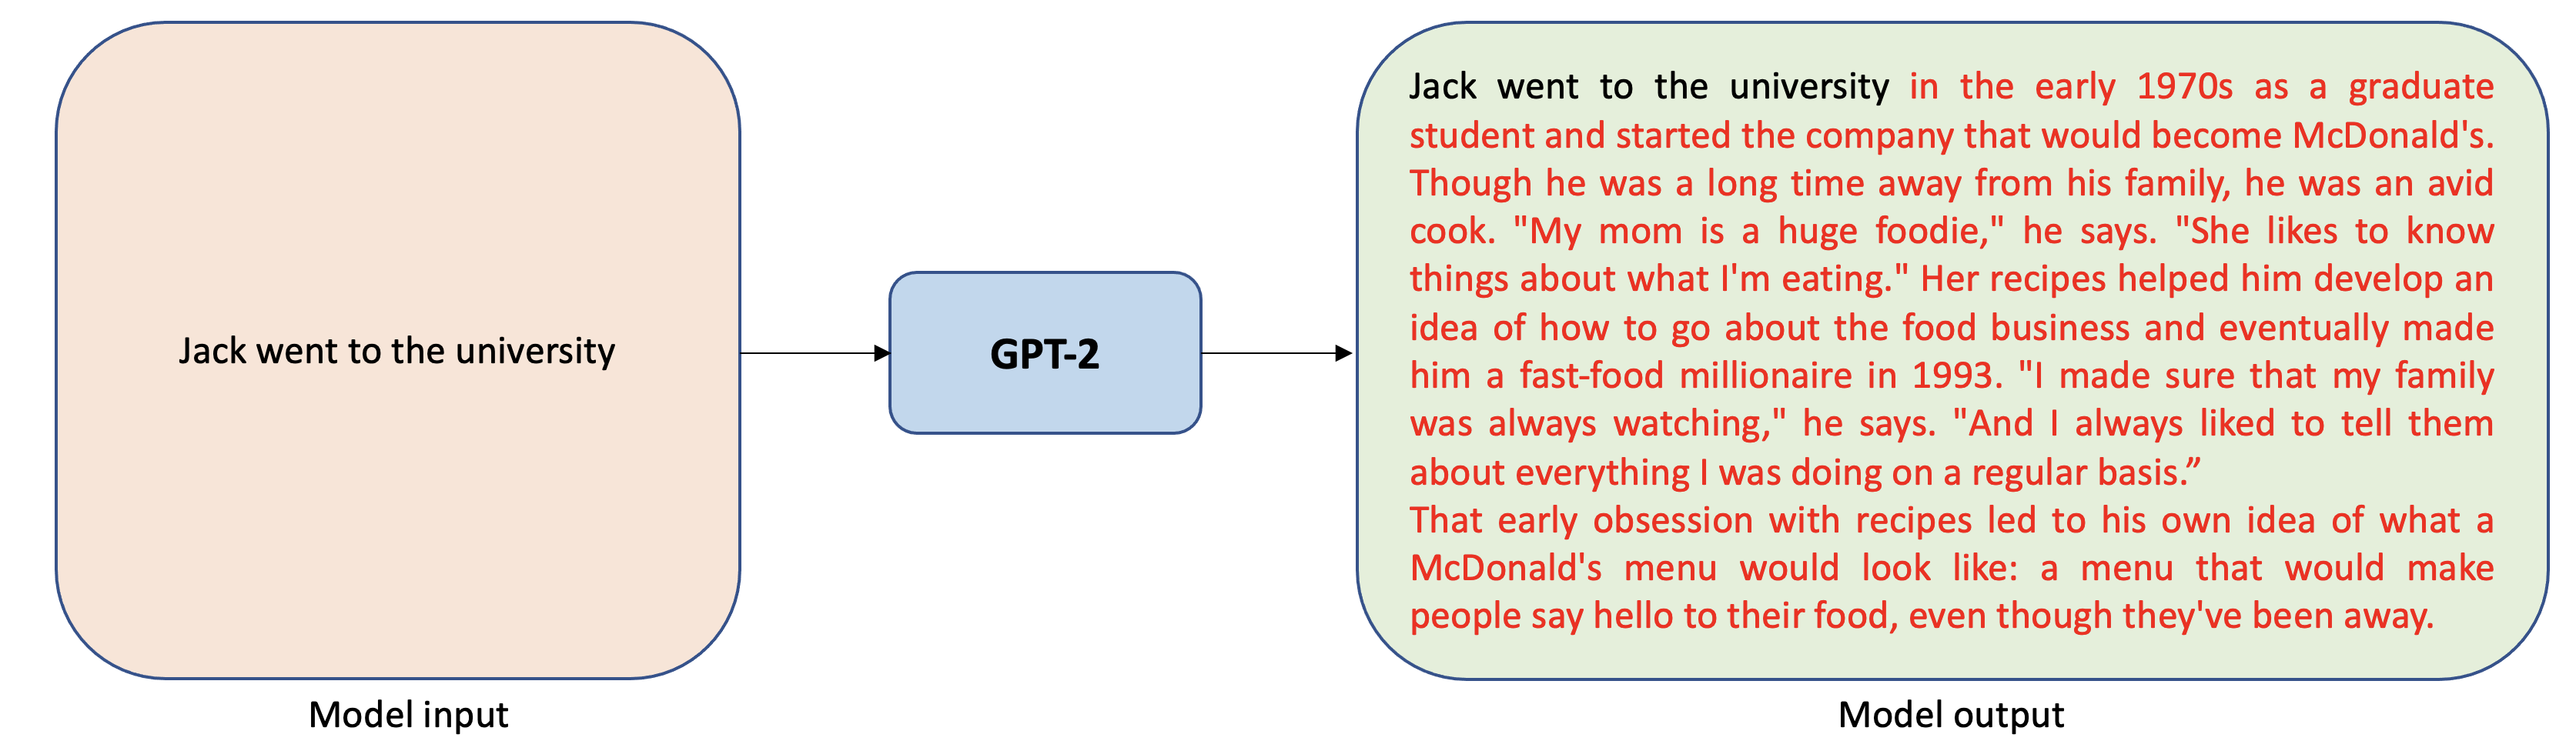
\includegraphics[width=0.9\textwidth]{./figuras/GPT2_text_generation.png}
    \source{\cite{RunTextGeneration2022}}
    \label{fig:gpt2_text_generation}
\end{figure}

Los \textit{grandes modelos de lenguaje} emplean la arquitectura \textit{Transformer} o derivados. Se entrenan con grandes cantidades de texto sin etiquetar, como libros, artículos de periódicos, páginas web, etc., realizándose este proceso en paralelo, lo que requiere una gran capacidad computacional. Sin embargo, una vez entrenados, estos modelos pueden ser utilizados para tareas de generación de texto, traducción automática, resumen de textos, etc. con una capacidad predictiva sorprendente. La Figura \ref{fig:llm_sizes} muestra una comparativa de los tamaños de los LLM más conocidos.

\begin{figure}[H]
    \caption{Gráfico comparativo de tamaños de LLM}
    \centering
    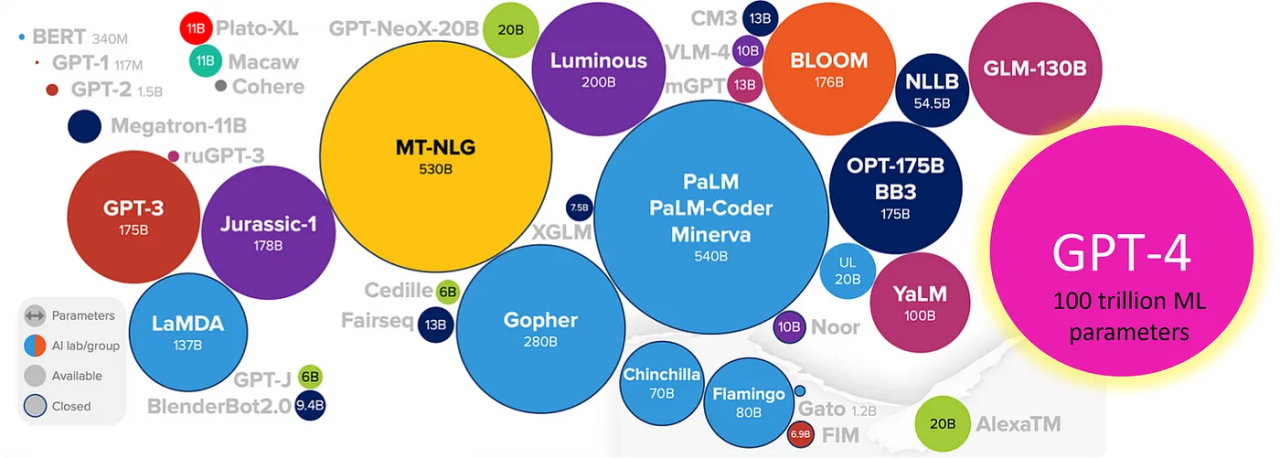
\includegraphics[width=0.9\textwidth]{./figuras/LLMs_sizes.png}
    \source{\cite{ChallengesAssociatedBuilding}}
    \label{fig:llm_sizes}
\end{figure}

\subsection{Modelos preentrenados}
\subsection{Ajuste fino de los modelos}
Bibliografía: \cite{chamandFinetuneYourClassifier2022}

\subsection{Hiperparámetros fijos del modelo}
Aquí hablaré de los hiperparámetros que definen la arquitectura del modelo que no se pueden modificar, como el número de capas, el número de cabezas de atención, etc., y que son fijos en el modelo. Especial atención se pondrá en el número de parámetros del modelo, que es el que determina el tamaño del modelo y su capacidad de generar textos, así como en la ventana de contexto, que es el número de tokens que el modelo tiene en cuenta para generar el siguiente token.

Precisamente el número de parámetros y la ventana de contexto son los hiperparámetros más importantes y críticos en términos computacionales y de efectividad. Cuanto más grande sea el modelo, más parámetros tendrá y más capacidad de generar textos tendrá. Sin embargo, también será más lento en la inferencia. Por otro lado, cuanto mayor sea la ventana de contexto, más tokens tendrá en cuenta el modelo para generar el siguiente token, y más coherentes serán los textos generados. Sin embargo, también será más lento en la inferencia.

Consideraciones interesantes sobre parámetros y ventana de contexto en \cite{gonzaloAsomandonosVentanaContextual2023}

\subsection{Hiperparámetros controlables por el usuario}
\label{sec:hiperparametros_controlables}
Hablar de la temperatura, top\_p, top\_k, ventana de contexto, número de tokens, etc. 

Se habla de la temperatura y su impacto en la generación de textos en \cite{holtzmanCuriousCaseNeural2020} y \cite{chamandFinetuneYourClassifier2022}

\cite{holtzmanCuriousCaseNeural2020} habla de la importancia de top\_p, en lo que denomina \textit{top\_k nucleus sampling}. Aunque es antiguo el paper, echar un ojo porque aclara bastante los conceptos.

Seguimos las explicaciones de \cite{rothmanTransformersNaturalLanguage2021}

Existen estudios centrados en la optimización de los hiperparámetros (los ya citados más arriba y \cite{wangCostEffectiveHyperparameterOptimization2023} y \cite{wangHyperparameterOptimizationAlgorithm2022})





\section{\textit{Prompting engineering}}

\label{sec:llm_tecnicas_prompting}

Se entiende por \textit{prompting} a la forma en la que se le pide a un modelo generativo una respuesta. En el caso de un LLM, que genere un texto \citep{LLMPromptingGuide}. El \textit{prompt} es el texto en lenguaje natural que el usuario presenta al LLM como input. El \textit{prompting} es un campo de investigación muy activo en la actualidad, y que ha dado lugar a numerosos estudios y publicaciones. El término \textit{prompting engineering} no está aceptado por la comunidad científica, aunque se pueden encontrar numerosos estudios científicos que acuñan esta denominación. En todo caso, para los propósitos de este trabajo, podemos entender por \textit{prompting engineering} el conjunto de técnicas que se utilizan para obtener mejores resultados en la generación de texto por parte de un LLM. 

\subsection{Técnicas más importantes de \textit{prompting engineering}}

En función del propósito de la interacción con sistemas basados en LLM, existen diferentes técnicas \textit{prompting} (ver Figura \ref{fig:prompting_engineering}). La forma más sencilla de \textit{prompting} es la denominaza \textit{zero-shot}, en la que el usuario presenta al LLM un \textit{prompt} y el LLM genera un texto de salida. En este caso, el LLM no ha sido entrenado para realizar una tarea específica, sino que ha sido entrenado con textos en lenguaje natural de propósito general. Sin embargo, el LLM puede generar un texto de salida que se corresponda con la tarea que el usuario quiere realizar. Por ejemplo, si el usuario presenta al LLM el \textit{prompt} <<\textit{¿Cuál es la capital de Francia}>>, el LLM puede generar un texto de salida como <<\textit{La capital de Francia es París}>>. En este caso, el LLM no ha sido entrenado como experto en geografía, pero ha sido entrenado con textos en lenguaje natural de propósito general, y es capaz de generar un texto de salida que se corresponde con la petición del usuario. La limitación de esta técnica es la del propio entrenamiento del LLM. Este no podrá generar nada en lo que no haya sido previamente entrenado.

\begin{figure}[H]
    \caption[Técnicas de \textit{prompting engineering}]{Técnicas de \textit{prompting engineering} aplicadas a problemas aritméticos.}
    \centering
    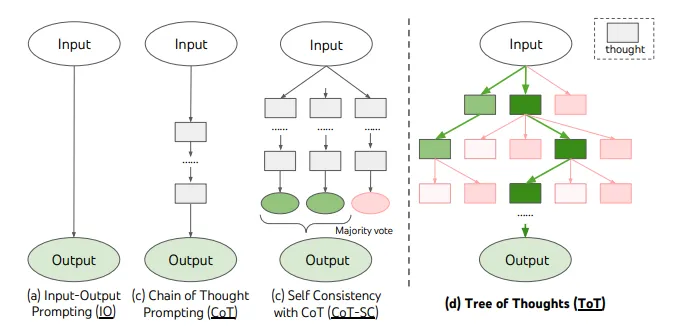
\includegraphics[width=0.9\textwidth]{./figuras/prompt_engineering_techniques.png}
    \source{\cite{bhavsarPromptEngineeringArithmetic2023}}
    \label{fig:prompting_engineering}
\end{figure}

\subsubsection{\textit{Few-shot prompting}}

Una primera técnica aplicable a un modelo de lenguaje es la de \textit{few-shot}, en la que el modelo recibe como input una serie de pares <<petición-respuesta>> más una petición a la cual ha de responder de forma análoga al contexto. Se presenta muy útil para tareas que requieren de cierto automatismo, como la generación de respuestas con un formato concreto, ya que en el input se muestra al LLM qué tipo de respuesta se requiere (ver Figura \ref{fig:few_shot_prompting}). De hecho, esta es la técnica que subyace tras las interfaces tipo \textit{chat} que se pueden encontrar en la mayoría de los LLM conversacionales. Si bien, fueron prentrenados para completar textos, pueden ser guiados por el \textit{few-shot prompting} a generar respuestas en un formato y personalidad concreta, ya que el modelo tenderá a repetir el estilo de los ejemplos pasados por contexto.

% \begin{figure}[H]
%     \caption[Técnica de \textit{few-shot prompting}]{Técnica de \textit{few-shot prompting}. El LLM recibe como input una serie de pares <<petición-respuesta>> más una petición a la cual ha de responder de forma análoga al contexto. En este caso, el LLM, con papel de <<asistente>>, ha de devolver el input del <<usuario>> con las letras invertidas. Sin embargo, nunca se le pide explícitamente que invierta las letras, sino que lo ha de inferir a partir de los ejemplos.}
%     \centering
%     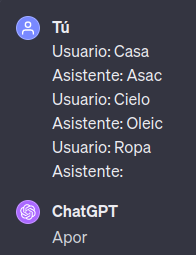
\includegraphics[width=0.2\textwidth]{./figuras/few_shot_prompting.png}
%     \source{Elaboración propia}
%     \label{fig:few_shot_prompting}
% \end{figure}


\begin{figure}[H]
    \caption[Técnica de \textit{few-shot prompting}]{Técnica de \textit{few-shot prompting}. El LLM recibe como input una serie de pares <<petición-respuesta>> más una petición a la cual ha de responder de forma análoga al contexto. En este caso, el LLM, con papel de <<asistente>>, ha de devolver el input del <<usuario>> con las letras invertidas. Sin embargo, nunca se le pide explícitamente que invierta las letras, sino que lo ha de inferir a partir de los ejemplos.}
    \centering
    \begin{subfigure}{.48\textwidth}
      \centering
      \begin{mdframed}
        Usuario: Casa
        \vspace{0.1cm}

        Asistente: Asac
        \vspace{0.1cm}

        Usuario: Ciclo
        \vspace{0.1cm}

        Asistente: Oleic
        \vspace{0.1cm}

        Usuario: Ropa
        \vspace{0.2cm}
      \end{mdframed}
    %   \caption{Csound}
    \end{subfigure}\hfill

    \vspace{0.2cm}

    \begin{subfigure}{.48\textwidth}
        \centering
        \begin{mdframed}
        Asistente: Apor
        \end{mdframed}
      \end{subfigure}\hfill

      \source{Elaboración propia}
      \label{fig:few_shot_prompting}
\end{figure}

\subsubsection{\textit{Chain of thoughts}}

Una técnica muy interesante es la denominada \textit{chain of thoughts}, que consiste en presentar al LLM un problema y pedirle que explique su razonamiento antes de dar la respuesta. Esta técnica se ha mostrado muy efectiva en especial en tareas de resolución de problemas aritméticos, ya que obliga al LLM a razonar antes de dar una respuesta, lo que lleva a una respuesta correcta en la mayoría de los casos \citep{weiChainofThoughtPromptingElicits2023}. Esta técnica pone en evidencia el hecho de que los LLM no razonan necesariamente su respuesta, a pesar de que ésta pueda resultar conviencente y pasar por correcta (ver \ref{sec:limitaciones_llm}). Por otra parte, esta técnica ha mostrado que el \textit{prompting} tiene un gran poder sobre el resultado de la inferencia en los modelos de lenguaje. 

La Figura \ref{fig:chain_of_thoughts} muestra un ejemplo de \textit{chain of thoughts} aplicado a un problema aritmético. Obsérvese cómo el LLM llega a la respuesta correcta sólo cuando se le incita a dar una explicación de su razonamiento. En este caso no se le ha pedido esta explicación explícitamente, sino a través de la técnica de \textit{few-shot prompting}. Las técnicas que se presentan a continuación pueden entenderse como derivaciones del principio de \textit{chain of thoughts}, en los cuales se fuerza un razonamiento explícito por parte del LLM antes de dar una respuesta.

\begin{figure}[H]
    \caption[Chain of thoughts]{\textit{Chain of thoughts}. En ambos ejemplos se plantea un problema aritmético a GPT-3. En (a), por medio de \textit{few-shot prompting}, se le pide una respuesta directa al problema. En (b), aplicando, además, la técnica de \textit{chain of thoughts}, se le pide que explique su razonamiento, lo cual lleva a una respuesta correcta. Se ha resaltado el texto correspondiente a los razonamientos.}
    \centering
    \begin{subfigure}{.48\textwidth}
      \centering
      \begin{mdframed}
        \setstretch{1}
        P: Roger tiene 5 pelotas de tenis. Compra 2 latas más de pelotas de tenis. Cada lata tiene 3 pelotas de tenis. ¿Cuántas pelotas de tenis tiene ahora?
        \vspace{0.2cm}

        R: La respuesta es 11.
        \vspace{0.2cm}

        P: La cafetería tenía 23 manzanas. Si usaron 20 para hacer el almuerzo y compraron 6 más, ¿cuántas manzanas tienen?
        \vspace{0.2cm}
      \end{mdframed}
    %   \caption{Csound}
    \end{subfigure}\hfill
    \begin{subfigure}{.48\textwidth}
      \centering
      \begin{mdframed}
        \setstretch{1}
        P: Roger tiene 5 pelotas de tenis. Compra 2 latas más de pelotas de tenis. Cada lata tiene 3 pelotas de tenis. ¿Cuántas pelotas de tenis tiene ahora?
        \vspace{0.2cm}

        R: \highlight{Roger comenzó con 5 pelotas. 2 latas de 3 pelotas de tenis cada una hacen 6 pelotas de tenis. 5 + 6 = 11.} La respuesta es 11.
        \vspace{0.2cm}

        P: La cafetería tenía 23 manzanas. Si usaron 20 para hacer el almuerzo y compraron 6 más, ¿cuántas manzanas tienen?
        \vspace{0.2cm}
      \end{mdframed}
    %   \caption{SuperCollider}
    \end{subfigure}

    \vspace{0.2cm}

    \begin{subfigure}{.48\textwidth}
        \centering
        \begin{mdframed}
        R: La respuesta es 29.
        \end{mdframed}
        \caption{\textit{Few-shot} para forzar una resolución directa de un problema aritmético. La respuesta es incorrecta.}
      \end{subfigure}\hfill
    \begin{subfigure}{.48\textwidth}
      \centering
      \begin{mdframed}
        \setstretch{1}
        R: \highlight{Comenzaron con 23 manzanas. Usaron 20, por lo que quedaron 23-20 = 3 manzanas. Compraron 6 más, por lo que ahora tienen 3+6 = 9 manzanas.} La respuesta es 9.
      \end{mdframed}
      \caption{\textit{Few-shot} con \textit{chain of thoughts} para provocar un razonamiento previo a la respuesta. La respuesta es correcta.}
    \end{subfigure}

    \source{\cite{weiChainofThoughtPromptingElicits2023}. Traducción propia.}
    \label{fig:chain_of_thoughts}
\end{figure}

\subsubsection{\textit{Self Consistency of Chain of Thoughts} (COT-SC)}

Esta técnica es una variante de \textit{chain of thoughts} que consiste en presentar al LLM un problema y pedirle que explique su razonamiento antes de dar la respuesta, pero en este caso se le pide realizar esta cadena de pensamientos en dos o más ocasiones, Tras ello se verifica qué respuesta es la más consistente. De este modo, no solo se provoca el razonamiento, sino y la posibilidad de llegar a un resultado desde diferentes puntos de vista. \cite{wangSelfConsistencyImprovesChain2023} muestra cómo esta técnica mejora a la de \textit{chain of thoughts} tanto en el terreno arimético como en el del razonamiento por sentido común. La Figura \ref{fig:cot_sc} muestra un ejemplo de esta técnica aplicada a un problema aritmético.

\begin{figure}[H]
    \caption[]{Esquema de los pasos en los que se divide la técnica \textit{Self Consistency of Chain of Thoughts}}
    \centering
    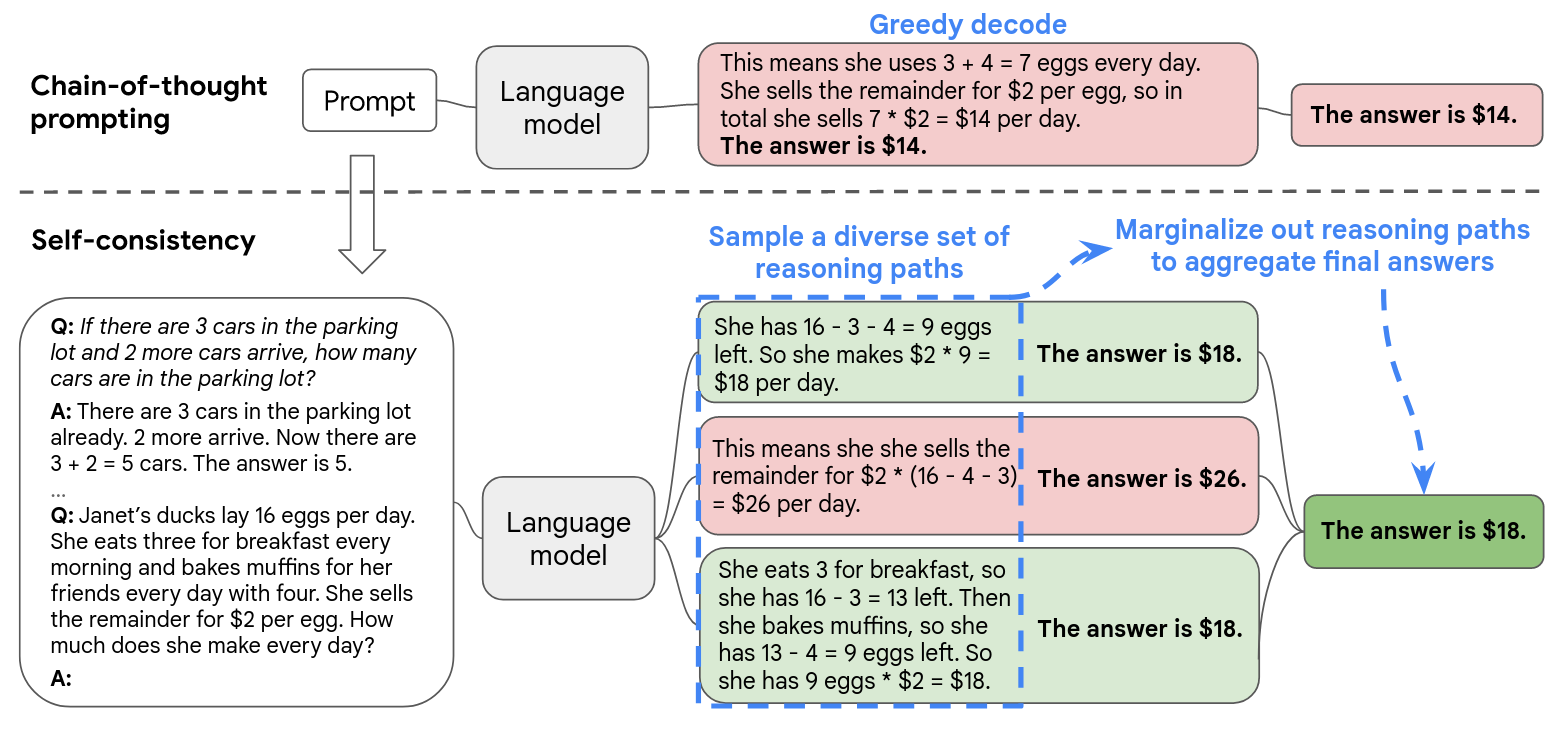
\includegraphics[width=0.9\textwidth]{./figuras/cot_sc.png}
    \source{\cite{wangSelfConsistencyImprovesChain2023}}
    \label{fig:cot_sc}
\end{figure}













El buen desempeño de los LLM en tareas de código de programación lleva a estudios como \cite{liStructuredChainofThoughtPrompting2023}, que propone un sistema de prompting que pide al LLM una reflexión explícita sobre la implementación a realizar, en una especie de pseudocódigo, que en un segundo paso será traducido al código final de programación. Este sistema de prompting se basa en la idea de que el LLM generará código de mayor calidad si se le permite <<pensar>> la respuesta antes de generarla. En este sentido, existen sobradas publicaciones que ponen de relieve la sensibilidad de los LLM a la forma en la que se le pide que procese la información (\textit{prompting}) y la correlación en la calidad de sus resultados \citep{zhouLeasttoMostPromptingEnables2023,weiChainofThoughtPromptingElicits2023,LLMPromptingGuide}.
 
\subsection{\textit{Retrieval-Augmented Generation} (RAG)}

Los modelos de lenguaje están prentrenados con grandes cantidades de texto de propósito general, lo que los hace capaces y hábiles en multiples campos sin necesidad de un entrenamiento específico (ver Figura \ref{fig:fundation_models_habilities}). Es posible, sin embargo, rentrenarlos con datos más concretos y precisos para una tarea específica (por ejemplo, con datos médicos, ingenieriles, con datos privados de una empresa, etc.). A este proceso se le conoce como \textit{fine-tuning} o <<ajuste fino>>. Sin embargo, el proceso de \textit{fine-tuning} de un LLM requiere de grandes cantidades de datos y tiempo de entrenamiento, algo que en este momento no está al alcance del usuario medio. Por ello, se están desarrollando técnicas que permitan a los usuarios aprovechar los modelos preentrenados para tareas específicas sin necesidad de \textit{fine-tuning}. Una de estas técnicas es \textit{Retrieval-Augmented Generation} (RAG) \citep{WhatRetrievalaugmentedGeneration2021}, que combina la recuperación de información con la generación de texto. Esta es una técnica que ofrece resultados muy notables en términos de eficacia y eficiencia frente al \textit{fine-tuning}. RAG consiste en pasar como contexto al LLM junto a la petición del usuario, una serie de fragmentos de texto que se corresponden semánticamente con la petición, y que se obtienen de una base de datos de documentos relacionados con la tarea a realizar. Esta base de datos puede ser de cualquier tipo, desde una base de datos de texto en lenguaje natural, hasta una base de datos de código de programación, pasando por una base de datos de partituras musicales, o una base de datos de audio, y representan la base de conocimiento extra (\textit{knowledge}) que el LLM manejará en sus interacciones con el usuario. Este sistema de \textit{prompting} está en la base actual de muchos productos relacionados con LLM, como Assistant o GPTs de OpenAI. La Figura \ref{fig:rag} muestra el esquema de funcionamiento de RAG. La base de datos del conocimiento del LLM es dividido en una primera fase en fragmentos más pequeños y analizados por el LLM para obtener una representación vectorial de cada uno de ellos. En una segunda fase, el LLM recibe el \textit{prompt} del usuario y lo analiza para obtener una representación vectorial. En una tercera fase, el LLM busca en la base de datos de fragmentos aquellos que tienen similitud vectoria (y, por ende, semántica) con el \textit{prompt} del usuario. En una cuarta fase, el LLM genera el texto de salida a partir del \textit{prompt} del usuario y de los fragmentos de texto recuperados de la base de datos. 



\begin{figure}[H]
    \caption[Esquema de funcionamiento de RAG]{Esquema de funcionamiento de RAG. El LLM recibe como input el \textit{prompt} del usuario y, como contexto, una serie de fragmentos de texto de la base de datos de conocimiento, que tienen similitud vectorial con el \textit{prompt} del usuario.}
    \centering
    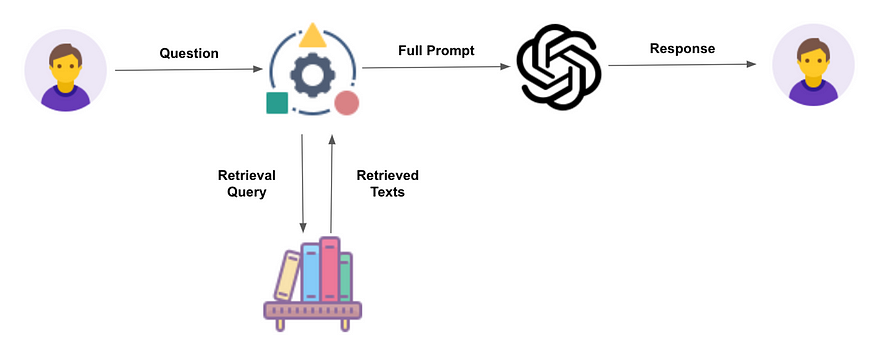
\includegraphics[width=0.9\textwidth]{./figuras/rag.png}
    \source{\cite{WhatRetrievalAugmented}}
    \label{fig:rag}
\end{figure}

Esta técnica, frente al \textit{fine-tuning}, ofrece una serie de ventajas, como la posibilidad de utilizar modelos preentrenados de propósito general, que son más eficientes y eficaces que los modelos entrenados para una tarea específica, y la posibilidad de utilizar bases de datos de conocimiento de gran tamaño, que son más fáciles de obtener que los grandes conjuntos de datos necesarios para el \textit{fine-tuning}. Además, la base de datos de conocimiento puede ser actualizada de forma independiente al modelo, lo que permite una mayor flexibilidad en el uso de los modelos. Por contra, el modelo no tiene conocimiento global de los contenidos de la base de datos, por lo que no puede realizar inferencias globales sobre ella, y la calidad de los resultados depende en gran medida de cómo se ha dividido su contenido en fragmentos y de la calidad de la representación vectorial de cada uno de ellos. Se ha probado un mayor rendimiento en técnicas combinadas de \textit{fine-tuning} para tareas específicas y RAG \citep{lewisRetrievalAugmentedGenerationKnowledgeIntensive2021}.


\subsection{\textit{prompting} versus \textit{fine-tuning}}

\subsection{Habilidades emergentes de los modelos de lenguaje}

\begin{figure}
    \caption{Habilidades de los \textit{Foundation Models} de OpenAI.}
    \centering
    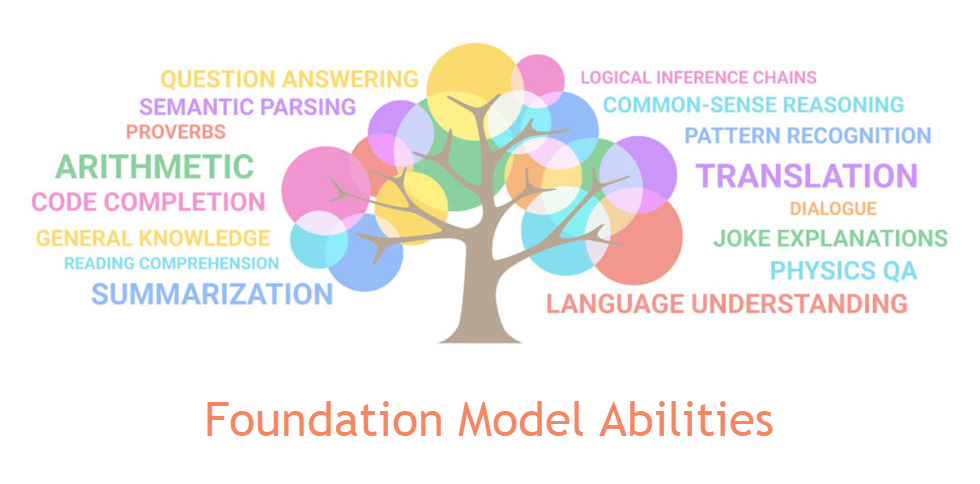
\includegraphics[width=0.8\textwidth]{./figuras/fundation_models_habilities.png}
    \source{\cite{GPT3RiseFoundation}}
    \label{fig:fundation_models_habilities}
\end{figure}


\section{Limitaciones conocidas de los LLM}
\label{sec:limitaciones_llm}
Ventana de contexto, sesgos, alucinaciones, dar la razón al usuario, 










